
\documentclass{article}
\usepackage{hyperref}
\usepackage{graphicx}
\usepackage[font=small,labelfont=bf]{caption}
\begin{document}

\title{Manual on construction and use of the Hashky}
\author{Hashky \href{mailto:hashkyinfo@gmail.com}{hashkyinfo@gmail.com}}
\maketitle

\begin{abstract}
This document is to provide description, instructions and philosophy of use of the Hashky. 

\end{abstract}


\section{Motivation}

Password strength is the most important element of maintaining effective security practices. A strong password must be far removed from the human lexicon, which is a property that will make it difficult to remember. Compounding this issue is the suggested practice of changing passwords often. Another property of a strong password is raw entropy content, which manifests itself as long length. This makes typing them time consuming and prone to error. All of these factors make strong passwords inconvenient for the average user.

The Hashky is a platform agnostic piece of hardware designed to overcome these problems. It generates and stores secure authentication entropy in an IC which contains a hardware random number generator and a secure EEPROM. The entropy is easily accessed using a small amount of user supplied entropy(a pin code), and presented using USB keyboard emulation.  

The original use case was for situations which requiring passwords with high entropy in situations where software password managers are not available. A prime case is an encrypted volume at boot; or a bios password. As early development progressed, it became apparent that such a device would be useful for the secure generation and storage of seed entropy for cryptocurrency wallets.  

In order to further increase security, the project was open-sourced, so that the code could be audited to avoid the threat of manufacturer or developer perpetrated compromise.  

\section{Features}

The Hashky is capable of generating three different styles of alphanumeric secrets and passwords. The formats are as follows: BIP39 pneumonic seedphrase, generic short alphanumeric password, IOTA wallet seeds. The generic short format is alphanumeric, lower and uppercase, as well as some special characters selected for maximum compatibility. 

The other formats are open standards and should be referenced in their respective white papers \cite{bip39,iota}. The BIP39 seedphrase is supported by many cryptocurrency wallets of various projects as a wallet recovery function.  


\begin{figure}
\centering
 \captionsetup{width=.7\linewidth}
\includegraphics[width=0.5\linewidth]{hashky.eps}
\caption{The Hashky incarnate, components labeled. The indicator LED is between the two boards, and can be witnessed through the gap labeled above. }
\label{fig:key}
\end{figure}

There are five buttons on the Hashky, labeled in Figure ~\ref{fig:key}. Buttons 1-4 are used for both input of user entropy and selection of password format. The fifth button labeled ENTER is used to mark the end of the sequence and initiate input of the password/secret. 

There is a secure element on the board, which is used to generate and securely store the entropy from which passwords are generated. The secure element contains a hardware random number generator and secure EEPROM that is resistant to physical tampering. For more details, refer to official datasheet of the Atmel ATSHA204. 

This device also has the function of the SHA256 hashing algorithm. The device can access the entropy for hashing, but is configured to preclude reading in plain text. This makes copying a configured Hashky impossible without physically compromising the advanced physical security features of the ATSHA204. 

The generic short format uses a set of $70$ characters and is of length $15$. This makes the entropy of this format $\log_2(70^{15})$, roughly $91$ bits. The code can easily be modified to use more characters. Some special characters are excluded in an effort to give maximum compatibility. It can be easily customised to the user's need without significantly changing the firmware.


\section{Features and use}


When buttons 1-4 have been actuated simultaneously, the device's indicator light will illuminate solid for a few seconds. This indicates that new personal entropy has been generated on the ATSHA204 and written to its EEPROM. Now your device contains your own personal unique entropy, and secrets generated are not dependent on any information known to any external entity. This can be done as many times as you like, but beware, there is no way to recover the state of the device after such a reset. The device must be powered up for this to work, so it will not happen in your pocket. 

Now, to generate/access passwords, the user begins by choosing the output format desired. This is done by pressing one of buttons 1-4. The corresponding formats for each button are:

\begin{enumerate}
\item  BIP39 pneumonic seedphrase \cite{bip39}
\item  BIP39 pneumonic seedphrase \cite{bip39}
\item  Generic 15 character alphanumeric and special character password
\item  IOTA wallet seeds \cite{iota}
\end{enumerate}


Following this selection, the user may input an arbitrary length base 4 sequence that can be thought of as a pin code or and address to each secret. The LED indicator will give a response during each actuation. Also buttons can be held down and actuations counted by observing the activity of the indicator LED(to allow reproducibility). After the desired sequence is entered, the ENTER button is pressed to finish the process and type the password into the host through USB keyboard emulation. This also resets the ephemeral state of the device, so that the same output will be achieved if we return to the output format selection step and reproduce the same sequence of button presses.

The default output is BIP39, so if the user simply hits enter without actuating buttons 1-4, a BIP39 output will be produced. 

The pin code itself should be thought of as a password and entropy. The first element of the code selecting the output format. 

\subsection{Philosophy of use}

The Hashky is a novel secure way to generate cryptocurrency wallets. It is very small(in physical size and memory) which makes it a bad candidate to carry malicious code. It is also open source and has a small codebase, so it can be easily audited. It is also fully deniable, as any input(pin code) to the device will produce a valid seed, so it is an excellent means of transportation for valuable seeds. The device also has no radios nor the capability to call home in any capacity. The connection being a purely physical one there is little chance of a MiTM attack, unless the host device is already compromised in some manner. 

In order to compromise a secret generated by the device, one must physically access your particular device and the relevant pin codes to access your secrets/passwords. If the device is stolen or otherwise placed in the attackers control, the key space is reduced but can only be accessed by entering pin codes into the device, unless the secure element is physically compromised in a hardware attack against the secure EEPROM. The pin codes are of arbitrary length, so in theory one may carry/generate a countably infinite number of passwords/wallet seeds with one Hashky.

Important secrets that are non-recoverable must be backed up by the user in a secure manner. It is the user's responsibility to guarantee that they will not be lost. 

The Hashky is only as secure as the device it is plugged into, you are still subject to keyloggers in a compromised host. 


\subsection{Good practices and tips}

\begin{itemize}
\item Use a USB extension cord to avoid damage to host USB ports when actuating tact switches.
\item Functionality on a tablet or phone is possible using an OTG adapter.
\item For extra security in the case that the device is stolen or lost, use a long pin code.
\item To use very long pin codes, hold buttons down and count the number of actuations by observing the LED response.
\item For use cases where the password can not be recovered, back it up by writing it down or printing it out and store it securely.
\item Remember it is only as secure as what you plug it into. This does not protect against keyloggers. 
\end{itemize} 


\section{Construction and initialization}

Physical construction of the Hashky is straight forward. Obtain all components on the bill of materials, including the Hashky "hat" PCB. Complete the PCB with the buttons and secure element. Now solder the hat PCB on top of the CJMCU beetle board with the pins. They will extend vertically, and must be trimmed after soldering. If you wish to use an ISP programmer for the firmware, you must leave them untrimmed until you have uploaded the firmware and tested the functionality. 

Once the Hashky has been physically constructed, the firmware must be uploaded. 

This is a two stage process. The first firmware is programmed to the device with either an ISP programmer or using the USB interface with the arduino bootloader. This firmware is called "init\_SHA". It contains routines which configure the secure element. This is a one-time process. After burning this firmware the device will be configured a few seconds after power-up and confirm this by emulating a USB keyboard and typing a confirmation text. This is very important for security as if the secure element is not properly configured, it will not make use of its secure features. 

In the main firmware "hashky\_firmware" there is a constant used to initialize the hashing process called "chal" on line 2326. It is not necessary, but good practice, to write some of your own entropy into this variable by changing around the hex digits.  Do not change the length of this variable. 

The firmware requires the two libraries in the firmware/libraries folder, so make them available to your arduino environment. 

The version of arduino used was 1.0.5+dfsg2-4. Some newer versions have serious bugs in parsing engine that will manifest in failure to compile the Hashky firmware. 

The main firmware is then written using either the USB interface with the arduino firmware or an ISP programmer. It is recommended to overwrite the arduino bootloader so that the device can not be accidentally reprogrammed during use. After the main firmware is written, the device is ready. 

The option of programming it over the USB interface using the arduino bootloader has been left for convenience and experimentation. 

The device can be re-initialized at any time by holding down keys 1-4 while the device is powered up. Upon success the LED will go solid then blink several times. This means new entropy has been written to the device. Remember this will overwrite any existing entropy so must be done with caution.


\subsection{Bill of materials}
\begin{itemize}
\item 5x 2 prong SMT tact switches TS-1236
\item 1x atmel atsha204, SOT23 form factor
\item 1x resistor 0805 4.7kohm-10kohm
\item 1x hashky hat board(included in this git)
\item 1x arduino CJMCU-beetle style board. Atmel Atmega32u4 or equivalent. Beware, there exists a board in this form factor with a different pinout. \ref{fig:cjmcu}
\end{itemize}


\begin{figure}
\centering
 \captionsetup{width=.7\linewidth}
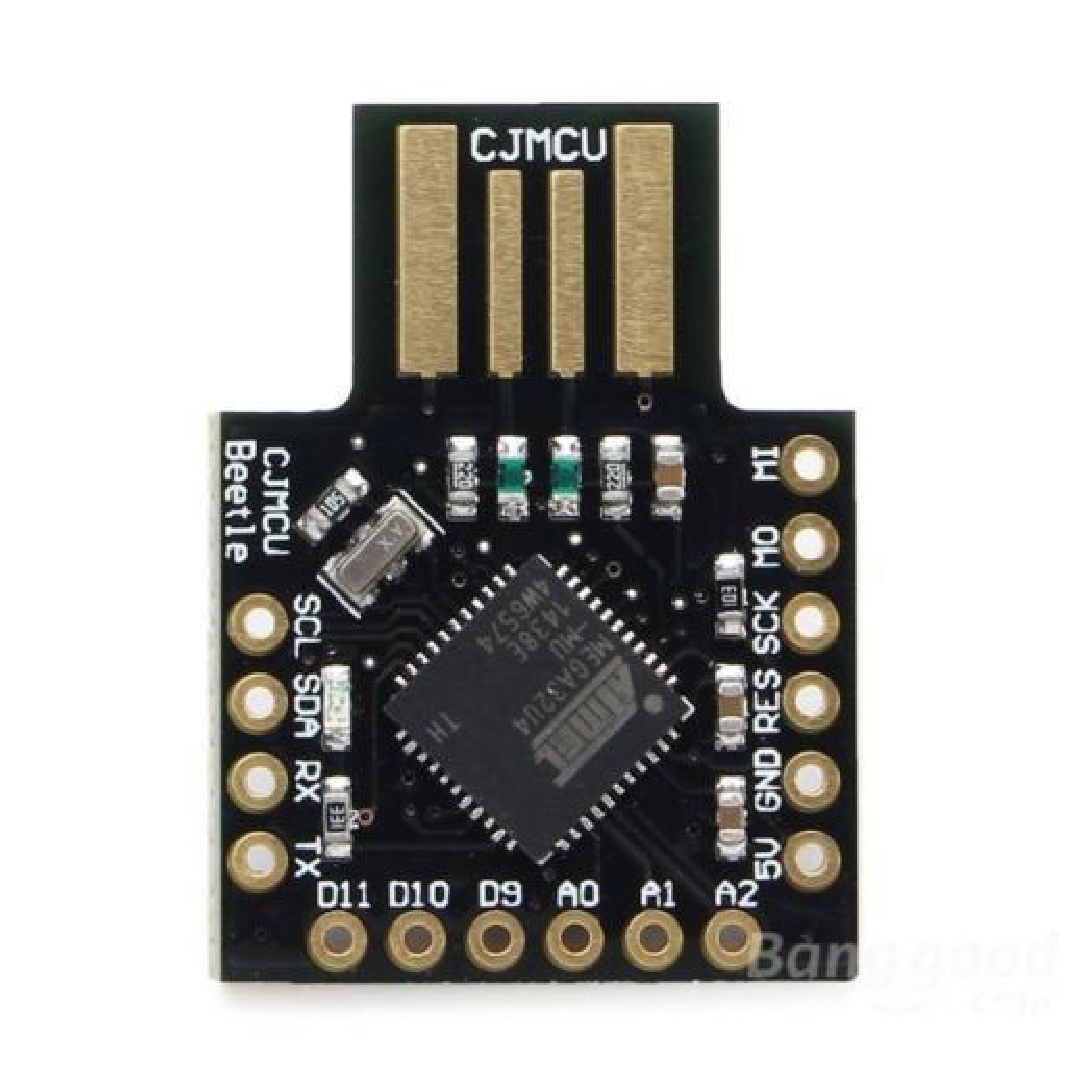
\includegraphics[width=0.5\linewidth]{cjmcubeetle.eps}
\caption{An image of the development board from the BOM. CJMCU-beetle, an Atmel Atmega32u4. }
\label{fig:cjmcu}
\end{figure}


\subsection{Troubleshooting}

If the secure element is not properly connected, it will return all 0s, so the outputs for IOTA seeds and standard passwords will be a string of As. The BIP39 output will be similar, an output containing only the word "ambient". 

The 3D printed case is attached by sliding the male USB region of the device into the opening on the side of the case, so that the entire board is diagonal to the bottom of the case. Then the side opposite to the USB is pushed down, snapping the board down into the case. The case is often very difficult to remove non-destructively after this has been done. The case can physically obstruct the insertion of the Hashky into some USB host ports enough to prevent connection of the data lines. This can be remedied with a USB extension cord. 

It is highly advisable to use a USB extension cord. This avoids causing damage as well as a temporary disconnect of the device during actuation of tact switches. This temporary disconnect can power cycle the device, causing a reset of the ephemeral state of the device, which will confound the pin code sequence being entered(but not damage the device or effect the secure element). 


\begin{thebibliography}{99}
\bibitem{bip39} BIP39 \href{https://github.com/bitcoin/bips/blob/master/bip-0039.mediawiki}{https://github.com/bitcoin/bips/blob/master/bip-0039.mediawiki}
\bibitem{iota} IOTA SUPPORT: Creating a new Seed/Wallet  \href{https://iotasupport.com/gui-newseed.shtml}{https://iotasupport.com/gui-newseed.shtml}
\end{thebibliography}

\end{document}
